\section*{Giratore Petin}
\begin{figure}[h]
  \centering
  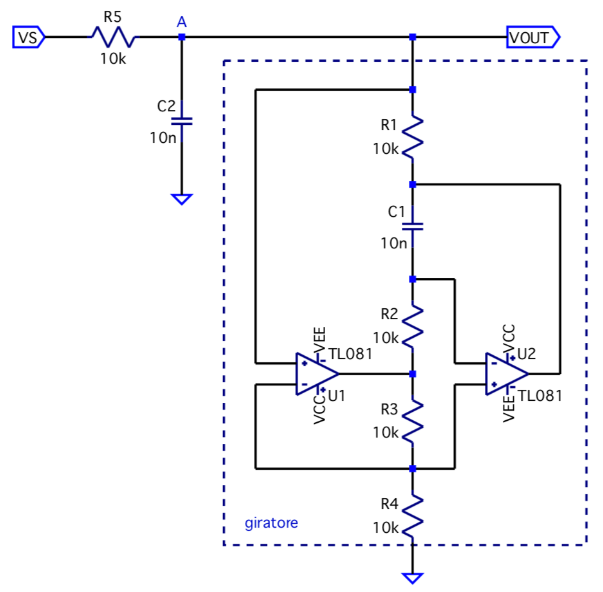
\includegraphics[width=0.4\textwidth]{src/images/petin.png}
\end{figure}

\begin{multicols}{2}
  \noindent\colorbox{orange}{
    \begin{minipage}{0.9\linewidth}
      \subsection*{Richiesta (a)}
      Sulla base di semplici considerazioni di natura qualitativa, verificare la caratteristica di filtro
      passa-banda studiando l'andamento di $V_{OUT}$ ai limiti del dominio in frequenza (verificando
      cio\'e che $V_{OUT} \to 0$ sia per $\omega \to 0$ che per $\omega \to \infty$).
    \end{minipage}
  }
  \subsection*{Risposta (a)}
  \begin{itemize}
  \item
    Per \textit{bassissime} frequenze il ramo del condensatore $C_2$ agisce da ``aperto'',
    nell'ipotesi di op-amp ideale e nel regime di operazione lineare per cui si applica il
    \textit{principio di corto-circuito virtuale} (si pu\'o fare nel limite di op-amp con guadagno
    finito, tutt'avia poi non sarebbe pi\'u un ``osservazione semplice'')
    \begin{equation*}
      V_{OUT} = V_{+U_1} = V_{-U_1} = \boxed{V_{+U_2} = V_{-U_2}}
    \end{equation*}
    tutt'avia \'e anche vero che
    \begin{equation*}
      \boxed{V_{-U_2}} = V_{U_1} \quad
      \boxed{V_{+U_2}} = V_{U_1}/2
    \end{equation*}
    di conseguenza
    \begin{equation*}
      \begin{cases}
        V_{OUT} = V_{U_1} / 2 \\
        V_{OUT} = V_{U_1}
      \end{cases} \implies \colorbox{blu}{\boxed{V_{OUT} = 0}}
    \end{equation*}
    
  \item
    Per \textit{altissime} frequenze il ramo del condensatore $C_2$ agisce da ``corto-circuito'', la tensione d'uscita
    $V_{OUT}$ \'e pari a quella della ``terra''.
    \begin{equation*}
      \colorbox{blu}{\boxed{V_{OUT} = V_{ground} = 0}}
    \end{equation*}
    
  \end{itemize}

  \noindent\colorbox{orange}{
    \begin{minipage}{0.9\linewidth}
      \subsection*{Richiesta (b)}
      Giustificare il valore misurato al punto 1d per il rapporto tra la tensione in uscita ad $U_1$ e
      $V_{OUT}$.
    \end{minipage}
  }
  \subsection*{Risposta (b)}
  La risposta \'e contenuta nell'ultimo passaggio della verifica di tensione nulla $V_{OUT} \to 0$: in realt\'a
  il primo vincolo del sistema di equazioni \'e valido in generale al di fuori dal limite $\omega \to 0$
  \begin{equation*}
    \colorbox{blu}{\boxed{V_{U_1}/V_{OUT} = 2}}
  \end{equation*}
  Questo risultato non dipende dal fatto che la frequenza sia di centro banda. \\

  \noindent\colorbox{orange}{
    \begin{minipage}{0.9\linewidth}
      \subsection*{Richiesta (c)}
      Assumendo per semplicit\'a $R_1=...=R_5=R=10~\text{kW}$, $C_1=C_2=C=10~\text{nF}$ e sulla base delle
      ipotesi di idealit\'a degli operazionali e di linearit\'a del circuito (quest'ultima verificata dalle
      misure precedenti), derivare un'espressione analitica dell'impedenza di ingresso del blocco
      identificato nello schema come "giratore" (in altri termini si immagini di scollegare quel
      blocco dal resto del circuito e di collegare il suo ingresso A ad un generatore di tensione
      sinusoidale e si calcoli il fasore della corrente erogata).
    \end{minipage}
  }
  \subsection*{Risposta (c)}
  Nell'ipotesi di op-amp ideale e nel regime di operazione lineare si applica il
  \textit{principio di corto-circuito virtuale} da cui \'e possibile calcolare la corrente che scorre
  attraverso il ramo di $R_4$
  \begin{equation*}
    I_4 = \frac{V_{OUT}}{R}
  \end{equation*}
  sempre per ipotesi di idealit\'a dell'op-amp gli ingressi invertenti non erogando corrente
  \begin{equation*}
    I_3 = I_4
  \end{equation*}
  da cui si ottiene la tensione del nodo in comune con l'uscita dell'op-amp $U_1$ mediante la KCL
  \begin{equation*}
    \begin{gathered}
      \frac{V_{U_1} - V_{OUT}}{R} = I_3 = I_4 = \frac{V_{OUT}}{R} \\ \implies
      V_{U_1} = 2V_{OUT}
    \end{gathered}
  \end{equation*}
  da cui si ottiene la corrente $I_2$
  \begin{equation*}
    I_2 = \frac{V_{OUT} - V_{U_1}}{R}
  \end{equation*}
  sempre per ipotesi di idealit\'a dell'op-amp gli ingressi invertenti non erogando corrente
  \begin{equation*}
    I_2 = I_{C_1}
  \end{equation*}
  da cui si ottiene la tensione del nodo in comune con l'uscita dell'op-amp $U_2$ mediante la KCL
  \begin{equation*}
    \begin{gathered}
      \frac{V_{OUT} - V_{U_1}}{R} = I_2 = I_{C_1} = sC(V_{U_2} - V_{OUT}) \\ \implies
      V_{U_2} = -\frac{1 - sRC}{sRC}V_{OUT}
    \end{gathered}
  \end{equation*}
  da cui si ottiene la corrente $I_1$, quindi finalmente l'impdedenza d'ingresso $Z_{in}$
  \begin{equation*}
    I_1 = \frac{V_{OUT} - V_{U_2}}{R} \implies \colorbox{blu}{\boxed{Z_{in} \equiv \frac{V_{OUT}}{I_1} = sR^2C}}
  \end{equation*}

  \noindent\colorbox{orange}{
    \begin{minipage}{0.9\linewidth}
      \subsection*{Richiesta (d)}
      Verificare che detta impedenza sia equivalente a quella di un'induttanza e di quest'ultima si
      calcoli il valore atteso.
    \end{minipage}
  }
  \subsection*{Risposta (d)}
  Un elemento di circuito induttivo ha un espressione fasoriale
  \begin{equation*}
    Z_L = j\omega L
  \end{equation*}
  l'impedenza equivalente trovata in precedenza pu\'o essere modellizata da un induttore con induttanza
  \begin{equation*}
    \colorbox{blu}{\boxed{L = R^2C}}
  \end{equation*}

  \noindent\colorbox{orange}{
    \begin{minipage}{0.9\linewidth}
      \subsection*{Richiesta (e)}
      Sostituendo il giratore con l'induttanza equivalente, giustificare qualitativamente la natura
      del filtro ed i risultati ottenuti al punto 1b sulla base della sua equivalenza con un circuito
      serie RLC.    
    \end{minipage}
  }
  \subsection*{Risposta (e)}
  Sostituendo il giratore con l'induttanza equivalente (messa a terra) si studia in maniera ancora
  pi\'u semplice il comportamento del circuito per valori di pulsazione estremali
  \begin{itemize}
  \item
    Per \textit{bassissime} frequenze il ramo con il condensatore si ``apre''
    e il circuito rimanente \'e un partitore di tensione con un resistore
    ed un induttore, ma il ramo con l'induttore si ``corto-circuita''
    di conseguenza la tensione d'uscita \'e pari alla terra.
  \item
    Per \textit{altissime} frequenze il ramo con l'induttore si ``apre''
    e il circuito rimanente \'e un partitore di tensione con un resistore
    ed un condensatore, ma il ramo con il condensatore si ``corto-circuita''
    di conseguenza la tensione d'uscita \'e pari alla terra.
  \end{itemize}
  il filtro realizzato esibisce le qualit\'a di un \textit{filtro passa banda}. \\

  \noindent\colorbox{orange}{
    \begin{minipage}{0.9\linewidth}
      \subsection*{Richiesta (f)}
      Determinare la funzione di trasferimento $A_V = V_{OUT}/V_S$ del filtro.
    \end{minipage}
  }
  \subsection*{Risposta (f)}
  Sostituendo il contenuto del blocco con un induttore, in virt\'u della KCL
  \begin{equation*}
    \frac{V_S - V_{OUT}}{R} = sCV_{OUT} + \frac{V_{OUT}}{sR^2C}
  \end{equation*}
  da cui si ottiene la funzione di trasferimento
  \begin{equation*}
    \colorbox{blu}{\boxed{A_V(s) \equiv \frac{V_{OUT}}{V_S} = \frac{sRC}{1 + sRC + s^2R^2C^2}}}
  \end{equation*}

  \noindent\colorbox{orange}{
    \begin{minipage}{0.9\linewidth}
      \subsection*{Richiesta (g)}
      Dall'espressione ottenuta dedurre le caratteristiche di centro-banda (frequenza centrale,
      guadagno massimo, sfasamento) e confrontarle con le misure di cui al punto 1b.
    \end{minipage}
  }
  \subsection*{Risposta (g)}
  Il guadagno si ottiene mediante la \ref{eq:da-tfunc-a-gain}
  \begin{equation}
    \label{eq:multivibratore-doppio-derivatore-gain}
    \colorbox{blu}{\boxed{G(\omega) = \frac{RC\omega}{\sqrt{(1 - R^2C^2\omega^2)^2 + (RC\omega)^2}}}}
  \end{equation}
  nell'ipotesi in cui $\omega \neq 0$, dividendo numeratore e denominatore per $RC\omega$, si nota che
  il guadagno \'e \textit{monotono decrescente} a meno del termine quadratico sotto radice
  \begin{equation*}
    G(\omega) = \frac{1}{\sqrt{1 + \left(\frac{1 - R^2C^2\omega^2}{RC\omega}\right)^2}}
  \end{equation*}
  perci\'o all'annulamento di quel termine il guadagno \'e massimo
    \begin{equation*}
    \begin{gathered}
      \colorbox{blu}{\boxed{\Omega = \frac{1}{RC}}} \\
      \colorbox{blu}{\boxed{\max_{\omega \in [0, +\infty)}G(\omega) = G(\Omega) = 1}}
    \end{gathered}
  \end{equation*}
  lo sfasamento lo si calcola mediante \ref{eq:da-tfunc-a-fase-reale-positivo}
  \begin{equation*}
    \colorbox{blu}{\boxed{\phi(\omega) = \arctan\left(\frac{1 - R^2C^2\omega^2}{RC\omega}\right)}}
  \end{equation*}

  \noindent\colorbox{orange}{
    \begin{minipage}{0.9\linewidth}
      \subsection*{Richiesta (h)}
      In maniera analoga determinare frequenze di taglio, larghezza di banda e fattore di merito
      del filtro e confrontare i valori ottenuti con le misure di cui al punto 1c.
    \end{minipage}
  }
  \subsection*{Risposta (h)}
  si calcola la pulsazione di taglio
  \begin{equation*}
    \begin{gathered}
      \left(\frac{RC\omega}{\sqrt{(1 - R^2C^2\omega^2)^2 + (RC\omega)^2}}\right)^2 = \frac{\max G(\omega)^2}{2} \\ \implies
      R^2C^2\omega^2 \pm RC\omega - 1 = 0 \\ \implies
      \colorbox{blu}{\boxed{\omega = \frac{\sqrt5 \pm 1}{2RC}}}
    \end{gathered}
  \end{equation*}
  dunque la larghezza di banda
  \begin{equation*}
    \colorbox{blu}{\boxed{\Delta\omega = \frac{1}{RC}}}
  \end{equation*}
  e il fattore di merito
  \begin{equation*}
    \colorbox{blu}{\boxed{Q = 1}}
  \end{equation*}
    In termini di frequenza
    \begin{itemize}
    \item La \textit{frequenza di taglio sinistra}: $\sim 984~\text{Hz}$
    \item La \textit{frequenza centrale}: $\sim 1591~\text{Hz}$
    \item La \textit{frequenza di taglio destra}: $\sim 2575~\text{Hz}$
    \end{itemize}
\end{multicols}
